\chapter{Estado da Arte e Trabalhos Relacionados}
\label{ch:3estado_da_arte}

Neste capítulo, apresenta-se o mapeamento da literatura realizado no âmbito desta pesquisa, conduzido por meio de uma \acrfull{rsl}, seguindo as diretrizes metodológicas propostas por \textcite{scannavino_revisao_2017}. O objetivo central desta revisão consiste em identificar, avaliar e sintetizar os principais estudos publicados sobre a aplicação de arquiteturas de microsserviços em sistemas de \acrfull{ia}, com ênfase especial em aspectos de orquestração e desempenho. Para tanto, foram estabelecidos protocolos rigorosos de busca, seleção e análise de trabalhos, delimitando-se o escopo temático e definindo critérios de elegibilidade que garantissem a relevância e a qualidade científica dos materiais incluídos.

A revisão concentra-se particularmente em investigações que abordam avaliações experimentais de desempenho, testes comparativos de protocolos e métricas de eficiência em comunicações entre serviços, assegurando que a análise aprofunde questões diretamente relacionadas aos objetivos desta dissertação. A \autoref{sec:3-rsl} detalha o processo de revisão sistemática, descrevendo as etapas percorridas, os critérios de inclusão e exclusão adotados e os resultados obtidos em cada fase. Na \autoref{sec:3-sintese-trabalhos}, procede-se à análise crítica dos trabalhos selecionados, discutindo suas contribuições, limitações e relações com o contexto experimental aqui proposto, de modo a posicionar esta pesquisa no estado da arte e justificar sua originalidade e relevância.

\section{Revisão Sistemática da Literatura}
\label{sec:3-rsl}

Baseando-nos nas técnicas apresentadas por \textcite{scannavino_revisao_2017} e nos objetivos e na área de estudo delimitados no \autoref{ch:2pilares}, formulamos algumas questões de pesquisa para nortear a revisão sistemática da literatura. Essas questões visam identificar trabalhos relevantes já publicados na área, que são considerados referências de estado da arte para esta pesquisa. Estas perguntas são:

\begin{enumerate}
    \item  Como orquestrar microsserviços de modelos de \gls{ia} generativa?
    \item  Quais técnicas e métodos são discutidos para a orquestração desses microsserviços?
    \item  Qual tecnologia é mais adequada para suportar uma alta demanda de trabalho na orquestração de microsserviços?
\end{enumerate}

\subsection{Estratégia de Busca}

\textbf{BASE DE DADOS}: A estratégia de busca foi planejada para cobrir as principais bases de dados acadêmicas e motores de busca reconhecidos nas áreas de Engenharia de Software e \acrfull{ia}, assegurando uma abrangente cobertura da literatura científica. As plataformas selecionadas, destacadas por sua relevância e pelo volume de publicações qualificadas, incluem:
\begin{itemize}
    \item ABCD PBI (\url{https://www.buscaintegrada.usp.br/}): portal de buscas integrado da rede de pesquisa da USP e demais parceiros incluindo CAPES e outras instituições internacionais.
    \item Science Direct (\url{www.sciencedirect.com}): Uma das maiores bases de dados de literatura científica e técnica, com forte presença em engenharia e computação.
    \item IEEE Xplore (\url{ieeexplore.ieee.org}): Base de dados do Institute of Electrical and Electronics Engineers, crucial para publicações em engenharia, eletrônica e computação.
\end{itemize}

\textbf{STRING DE BUSCA}: A estratégia de busca foi construída a partir de um conjunto de palavras-chave em inglês e português, selecionadas para alinhar-se diretamente ao escopo desta dissertação. Utilizando operadores booleanos (AND, OR), buscou-se equilibrar abrangência e especificidade, refinando os resultados para o tema central — desempenho e orquestração de microsserviços em sistemas de \acrfull{ia} aplicados ao setor financeiro. Essa abordagem permitiu capturar a literatura mais relevante, majoritariamente internacional, sem perder de vista contribuições regionais significativas. As strings incluíram combinações como:

\begin{itemize}
\item "microservices" AND "AI models" AND "communication" AND ("benchmark" OR "comparison" OR "study")
\item "microservices" AND "orchestration" AND ("REST" OR "gRPC" OR "Apache Thrift") AND "benchmark"
\item "conversational agents" AND "microservices architecture"
\item "microservices" AND "AI models" AND "financial"
\end{itemize}

\textbf{RESULTADOS INICIAIS}: Estabeleceu-se como critério de triagem inicial a análise de \textbf{títulos e resumos (abstracts)} dos estudos recuperados pelas strings de busca, complementado por um filtro temporal que abrangeu o período de 2020 a 2025 para garantir a contemporaneidade dos trabalhos selecionados. Esta estratégia permitiu capturar as evoluções mais recentes nas tecnologias de microsserviços e \gls{ia}. Do volume inicial de documentos identificados, procedeu-se à eliminação de duplicatas, resultando em um corpus preliminar de \textbf{278 publicações únicas} para avaliação de elegibilidade nas etapas subsequentes.


\subsubsection{Critérios de Elegibilidade e Seleção}

Após a escolha das bases dados e definição das strings de busca, definiu-se um processo de filtragem e seleção dos trabalhos. Este processo de seleção dos estudos seguiu 4 etapas detalhadas a seguir, assegurando a inclusão apenas dos trabalhos mais relevantes e de alta qualidade científica:
\begin{enumerate}
\item \textbf{Identificação}: Nesta fase inicial, foram realizadas as buscas nas bases de dados utilizando as strings de pesquisa definidas. O objetivo foi coletar o maior número possível de documentos potencialmente relevantes.
\item \textbf{Triagem}: Os resultados brutos foram armazenados em uma ferramenta de gestão de referências chamada Zotero\footnote{Disponível em: \url{https://zotero.org/}. Acesso em: 29 ago. 2025.} para facilitar a organização. Em seguida, as duplicatas foram removidas. Uma primeira filtragem foi realizada através da leitura dos títulos, descartando artigos que claramente não se alinhavam ao tema. Além disso, apenas artigos publicados em periódicos avaliados por pares foram selecionados, demonstrando assim a relevância já posta à prova por outros pesquisadores.
\item \textbf{Seleção Inicial}: Os títulos e resumos dos documentos restantes foram lidos para uma avaliação mais aprofundada da relevância. Nesta etapa, foram selecionados os estudos que apresentavam uma possível interseção com os objetivos e questões de pesquisa, mesmo que de forma preliminar.
\item \textbf{Seleção Final}: A leitura completa dos artigos selecionados na etapa anterior foi realizada para verificar a interseção direta e aprofundada com os objetivos e questões de pesquisa desta dissertação. A qualidade metodológica e a contribuição científica de cada estudo foram avaliadas rigorosamente.
\end{enumerate}

\begin{table}[H]
\centering
\caption{Resultados das buscas utilizando os termos nas fontes definidas}
\begin{tabularx}{\textwidth}{|c|X|c|c|c|}
\hline
\textbf{Ordem} & \textbf{Termos da Pesquisa} & \textbf{PBi} & \textbf{IEEEx} & \textbf{Science Direct} \\
\hline
1 & "microservices" AND "AI models" AND "communication" AND ("benchmark" OR "comparison" OR "study") & 218 & 4 & 0 \\
\hline
2 & "microservices" AND "orchestration" AND ("REST" OR "gRPC" OR "Apache Thrift") AND "benchmark" & 195 & 2 & 2 \\
\hline
3 & "conversational agents" AND "microservices architecture" & 12 & 0 & 2 \\
\hline
4 & "microservices" AND "AI models" AND "financial" & 86 & 3 & 1 \\
\hline
\multicolumn{2}{|r|}{\textbf{Total}} & \textbf{511} & \textbf{9} & \textbf{5} \\
\hline
\end{tabularx}
\label{tab:3-total-rsl}
\vspace{-0.3cm}
{\raggedright \footnotesize Fonte: Elaborado pelo autor.\par}
\end{table}


\textbf{Etapas}: As etapas para seleção dos estudos foram aplicados em diferentes etapas do processo de revisão:
\begin{itemize}
\item \textbf{Etapa inicial de buscas}: Os filtros de \textit{período (2020-2025)} e \textit{idioma (inglês ou português)} foram aplicados diretamente nas plataformas de busca durante a recuperação inicial dos documentos.

\item \textbf{Triagem por título e resumo}: Nestas etapas, avaliou-se preliminarmente a \textit{abordagem temática}, selecionando estudos que tratassem de aplicação de microsserviços em sistemas de \gls{ia} ou assistentes virtuais.

\item \textbf{Leitura integral}: A \textit{ênfase em aspectos específicos} (desempenho, orquestração, escalabilidade ou desafios de comunicação) foi criteriosamente verificada apenas através da leitura completa dos artigos, constituindo-se no filtro mais refinado do processo.
\end{itemize}

Foram excluídos os trabalhos que não se enquadravam no escopo, como artigos sobre \acrfull{ia} sem relação com microsserviços ou microsserviços que não abordassem desempenho ou orquestração. Além disso, consideraram-se não elegíveis os artigos duplicados, revisões sistemáticas ou surveys, priorizando-se estudos primários empíricos, ou aqueles que não apresentassem conteúdo científico revisado por pares, como preprints não revisados, postagens de blogs sem autoria acadêmica e whitepapers sem rigor científico.

\begin{figure}[H]
\centering
\caption{Processo de Revisão Sistemática da Literatura (Adaptado de \textcite{scannavino_revisao_2017})}
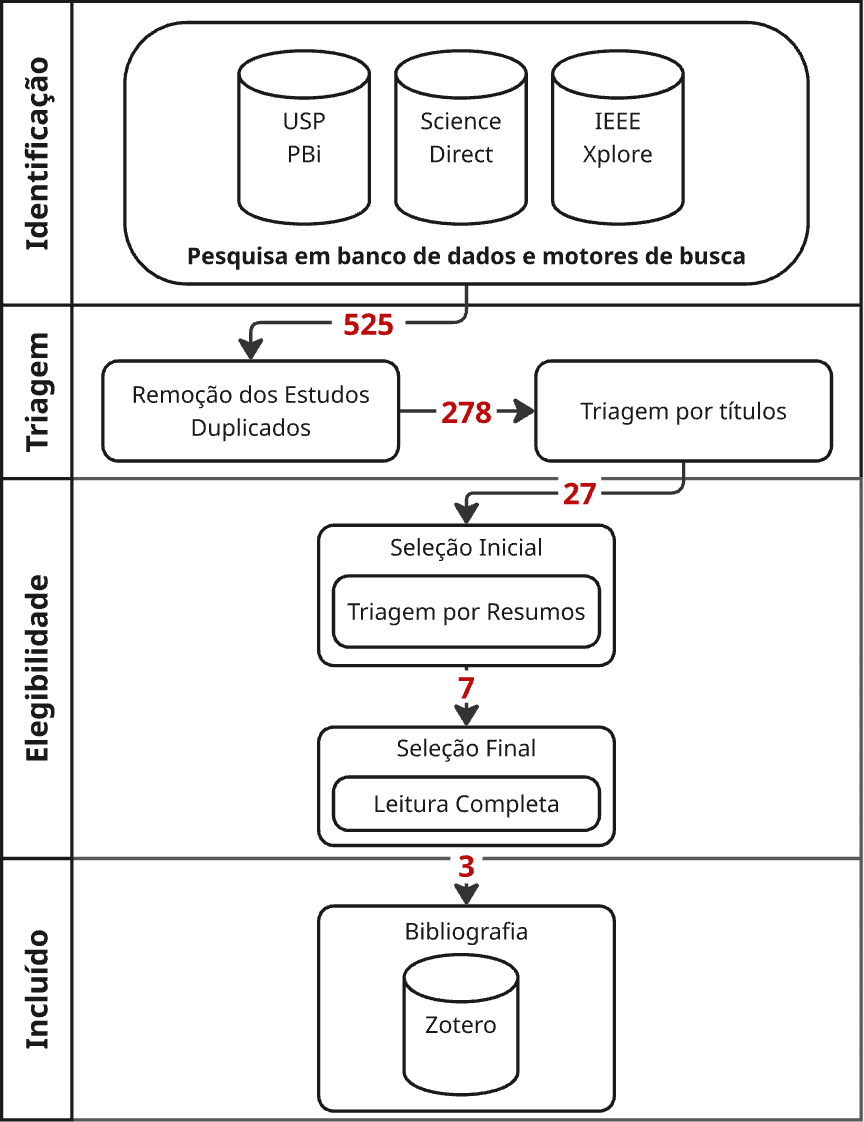
\includegraphics[width=0.65\textwidth]{imagens/3-revisao-literatura.png} 
\label{fig:rsl_process}
{\par \raggedright \footnotesize Fonte: Elaborado pelo autor.}
\end{figure}

A \autoref{fig:rsl_process} mostra o processo de seleção e triagem de documentos, que abrange desde a identificação inicial até a inclusão final. Por meio de métodos automatizados com o Zotero, o conjunto inicial foi reduzido a 278 documentos. A revisão dos títulos resultou na identificação de 27 estudos possivelmente relacionados ao tema. A análise dos títulos e resumos refinou a seleção para 7 estudos, dos quais 3 foram escolhidos após leitura aprofundada, devido à sua relevância direta para a pesquisa e ao seu destaque em relação aos demais artigos selecionados. Os números totais podem ser visualizados na \autoref{tab:3-total-rsl}.

A próxima seção examina os três artigos finais selecionados mediante uma análise crítica organizada em quatro dimensões principais: metodologia experimental (ambiente, ferramentas e cenários de teste), métricas de desempenho (latência, throughput, uso de recursos), motivação e objetivos, e conclusões e contribuições para a área. Essa abordagem multidimensional é estrategicamente alinhada aos objetivos desta pesquisa, uma vez que o exame detalhado das metodologias oferece insights para o desenho de nosso próprio ambiente de testes, a comparação das métricas possibilita a seleção das variáveis mais relevantes, a compreensão das motivações auxilia no posicionamento contextual de nossa contribuição, e a análise das conclusões fornece parâmetros comparativos para interpretar nossos resultados à luz do estado da arte. Dessa forma, esta seção não apenas sintetiza o conhecimento existente e estabelece um diálogo crítico entre os trabalhos identificando convergências e lacunas metodológicas, mas também fundamenta as escolhas metodológicas e analíticas adotadas neste trabalho.

\section{Síntese dos Principais Trabalhos Relacionados}
\label{sec:3-sintese-trabalhos}
% -- Niswar 2024
\subsection{Performance evaluation of microservices communication with \acrshort{rest}, \acrshort{graphql}, and \acrshort{grpc} \cite{niswar_performance_2024}}
\label{sec:3-niswar}

A pesquisa de \textcite{niswar_performance_2024} propõe uma avaliação e comparação abrangente do desempenho de três protocolos de comunicação amplamente utilizados em arquiteturas de microsserviços: \gls{rest}, \acrshort{graphql} e \gls{grpc}. O estudo concentra-se na troca de dados, abordando cenários de recuperação de dados planos e aninhados, com o objetivo de fornecer insights valiosos para que desenvolvedores e arquitetos possam otimizar a escolha dos protocolos de comunicação, considerando casos de uso e cargas de trabalho específicas.

O desafio da comunicação eficiente entre esses serviços independentes é um ponto central do trabalho. Embora os autores apontem o \gls{rest} como o método mais popular para troca de dados, eles argumentam que este protocolo apresenta desvantagens, como o over-fetching (recuperação de mais dados do que o necessário) e o under-fetching (recuperação de dados insuficientes, o que exige requisições adicionais). Nesse contexto, o \acrshort{graphql} surge como uma alternativa para superar tais ineficiências, permitindo que os clientes especifiquem exatamente os dados necessários. Já o \gls{grpc}, segundo os autores, destaca-se por sua abordagem eficiente e versátil na comunicação entre serviços distribuídos, utilizando o protocolo \acrshort{http}/2, que suporta streaming de dados e simplifica chamadas de procedimento remoto em diversas linguagens de programação.

Para realizar a avaliação, os autores estabeleceram um ambiente experimental composto por três microsserviços implementados em contêineres, cada um com um banco de dados Redis para cache em memória e MySQL para armazenamento persistente. O estudo utilizou dados de um Sistema Integrado de Informação Educacional, focando especificamente nas informações sobre o perfil dos professores e em seus históricos educacionais, abrangendo dados planos e aninhados. A metodologia de avaliação de desempenho empregou o Apache JMeter\footnote{Disponível em \hyperref[https://jmeter.apache.org]{https://jmeter.apache.org}} para simular testes de carga de \gls{api}, coletando métricas-chave como tempo de resposta e utilização da CPU. Foram realizadas duas abordagens de avaliação: requisições concorrentes e requisições consecutivas, com o número de requisições variando de 100 a 500, a fim de simular diferentes níveis de carga, conforme \autoref{fig:2-niswar-1}.

\begin{figure}[H]
    \caption{Cenário proposto por \textcite{niswar_performance_2024}}
    \label{fig:2-niswar-1}
    \centering
    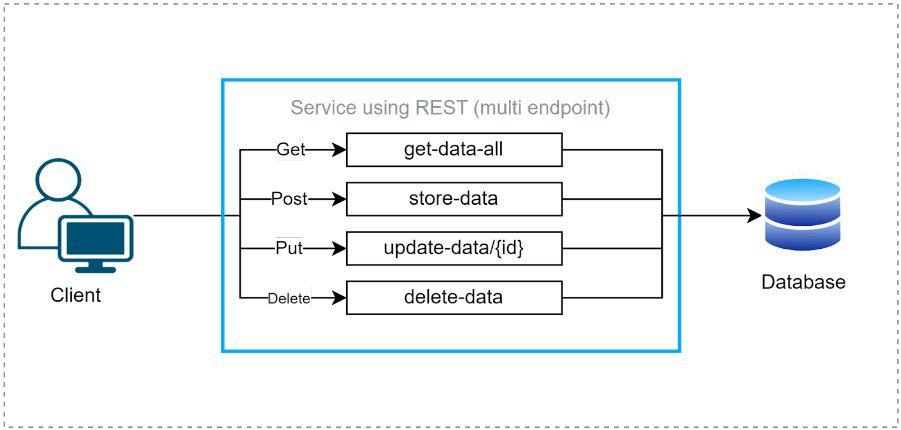
\includegraphics[width=0.75\linewidth]{imagens/niswar-1-enviroment.jpg}    
    {\par \raggedright \footnotesize Fonte: \textcite{niswar_performance_2024}.\par}
\end{figure}

Nos testes de requisições concorrentes, o tempo de resposta médio configurou-se como uma métrica crucial. Tanto para a recuperação de dados planos quanto aninhados, o \gls{grpc} demonstrou consistentemente tempos de resposta significativamente inferiores aos observados com \gls{rest} e \acrshort{graphql}. Por exemplo, para 100 requisições de dados planos, o \gls{grpc} foi aproximadamente 5 vezes mais rápido que o \gls{rest} e 16 vezes mais rápido que o \acrshort{graphql}. Essa vantagem de desempenho do \gls{grpc} manteve-se e intensificou-se à medida que o número de requisições aumentava, como pode ser observado nas figuras \ref{fig:2-niswar-time-flat} e \ref{fig:2-niswar-time-nested}.

Os resultados reforçam a eficiência do \gls{grpc} tanto para estruturas de dados simples quanto complexas e sob diferentes cargas, atribuída pelos autores ao uso do protocolo \acrshort{http}/2 e à serialização binária via Protocol Buffers.

\begin{figure}[htb]
  \centering
  \begin{minipage}[t]{0.48\linewidth}
    \caption{Tempos de respostas dos microsserviços com dados Flat}
    \label{fig:2-niswar-time-flat}
    \centering
    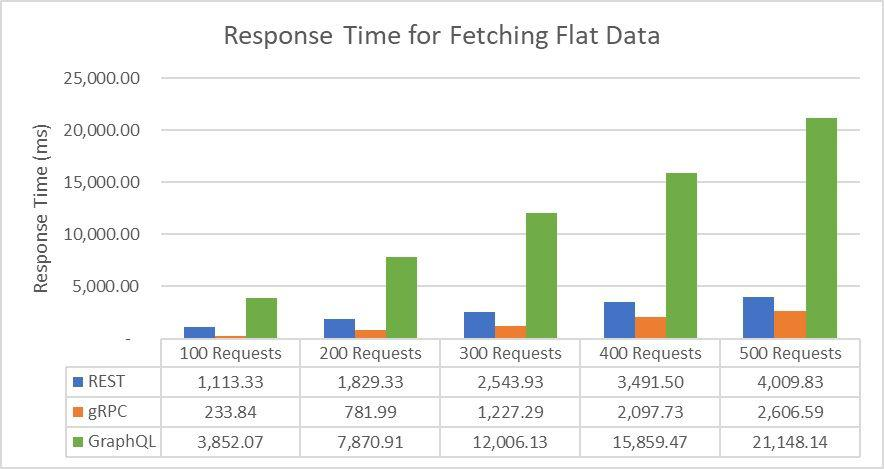
\includegraphics[width=\linewidth]{imagens/niswar_time_flat.jpg}    
    {\par \raggedright \footnotesize Fonte: \textcite{niswar_performance_2024}.\par}
  \end{minipage}%
  \hfill
  \begin{minipage}[t]{0.48\linewidth}
    \caption{Tempos de respostas dos microsserviços com dados Aninhados}
    \label{fig:2-niswar-time-nested}
    \centering
    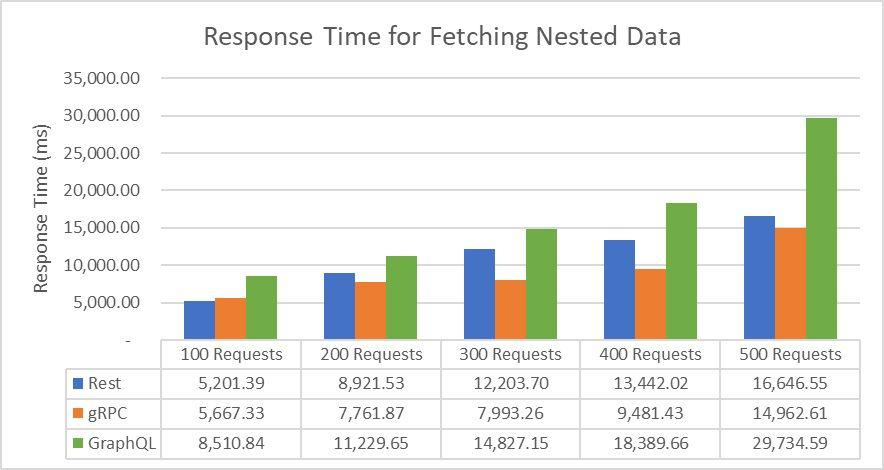
\includegraphics[width=\linewidth]{imagens/niswar_time_nested.jpg}    
    {\par \raggedright \footnotesize Fonte: \textcite{niswar_performance_2024}.\par}
  \end{minipage}
\end{figure}

Em relação à utilização da CPU, os resultados revelaram diferenças notáveis entre os protocolos, como ilustrado nas figuras \ref{fig:2-niswar-cpu-flat} e \ref{fig:2-niswar-cpu-nested}. Para a recuperação de dados planos, o protocolo \gls{rest} apresentou a menor utilização média da CPU, enquanto o \gls{grpc} mostrou consumo ligeiramente superior, porém ainda eficiente. Em contraste, o \acrshort{graphql} demonstrou uma utilização de CPU consideravelmente mais alta, frequentemente superando 100\%, o que, de acordo com os autores, indica uma demanda de recursos intensiva devido à complexidade inerente à análise e processamento de suas queries flexíveis.

Para a recuperação de dados aninhados, a tendência manteve-se semelhante: \gls{rest} e \gls{grpc} preservaram perfis de consumo mais eficientes, enquanto o \acrshort{graphql} novamente exigiu o maior esforço computacional, atingindo picos de utilização próximos a 180\% em cenários de maior carga. Esses padrões são visíveis nas figuras \ref{fig:2-niswar-cpu-flat} e \ref{fig:2-niswar-cpu-nested}, que detalham o comportamento dos protocolos sob diferentes volumes de requisições e complexidade de dados.

\begin{figure}[htb]
  \centering
  \begin{minipage}[t]{0.48\linewidth}
    \caption{Uso de CPU dos microsserviços com dados Flat}
    \label{fig:2-niswar-cpu-flat}
    \centering
    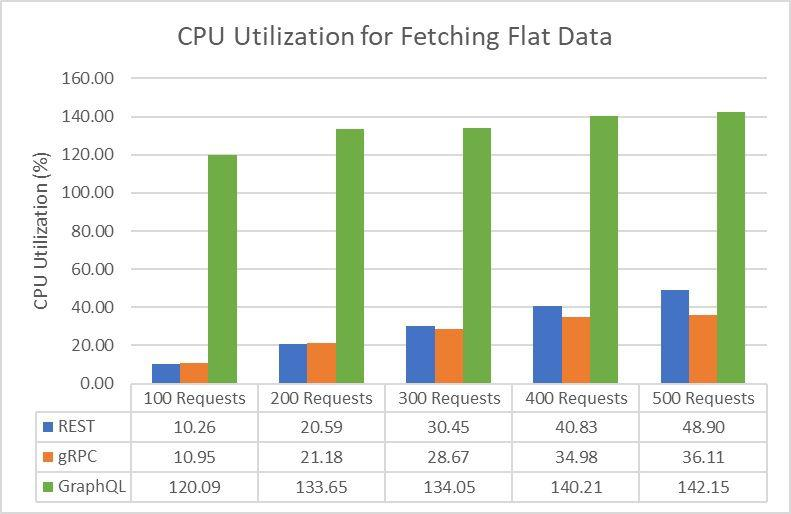
\includegraphics[width=\linewidth]{imagens/niswar_cpu_flat.jpg}    
    {\par \raggedright \footnotesize Fonte: \textcite{niswar_performance_2024}.\par}
  \end{minipage}%
  \hfill
  \begin{minipage}[t]{0.48\linewidth}
    \caption{Uso de CPU dos microsserviços com dados Aninhados}
    \label{fig:2-niswar-cpu-nested}
    \centering
    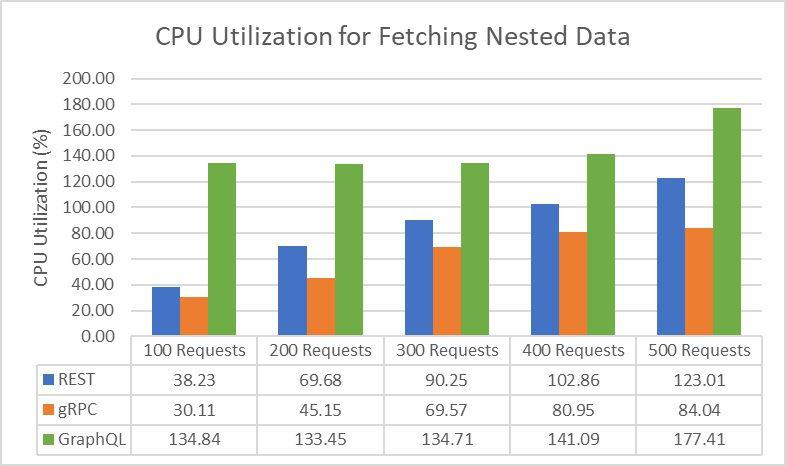
\includegraphics[width=\linewidth]{imagens/niswar_cpu_nested.jpg}    
    {\par \raggedright \footnotesize Fonte: \textcite{niswar_performance_2024}.\par}
  \end{minipage}
\end{figure}

A avaliação de requisições consecutivas, realizada durante cinco minutos e variando de 100 a 500 requisições, corroborou os achados dos testes concorrentes. O \gls{grpc} manteve-se como o protocolo com o tempo de resposta mais rápido para ambos os tipos de dados (flat e aninhados), evidenciando consistência sob diferentes padrões de carga. A capacidade do \gls{grpc} de utilizar o protocolo \acrshort{http}/2, que apresenta recursos como multiplexação (que permite múltiplas requisições sobre uma única conexão) e serialização binária eficiente (Protocol Buffers), é destacada pelos autores como o principal fator de seu desempenho superior em comparação ao \gls{rest} e ao \acrshort{graphql}.

\subsubsection{Resumo do Estudo}

Em suma, o estudo de \cite{niswar_performance_2024} conclui que o \gls{grpc} supera o \gls{rest} e o \acrshort{graphql} em termos de tempo de resposta, configurando-se como a escolha mais eficiente para comunicação em microsserviços que demandam baixa latência. Por outro lado, o \gls{rest} demonstrou menor utilização da CPU em alguns cenários, o que pode ser um fator relevante em ambientes com restrições de recursos. Embora o \acrshort{graphql} ofereça flexibilidade na recuperação de dados, resulta em maior consumo de CPU e aumento no tempo de resposta. As descobertas proporcionam insights práticos para a escolha de protocolos de \gls{api} em ambientes de microsserviços, levando em consideração os requisitos específicos de cada caso de uso e carga de trabalho.
% -- Maulana 2022
\vspace{\fill}
\subsection{Design and Testing on Migration of Remiss-Supply in Banking System to Microservice Architecture \cite{maulana_design_2022}}

\label{subsec:maulana_design}

\textcite{maulana_design_2022} apresentam um estudo focado na migração arquitetural de um sistema bancário monolítico para uma arquitetura de microsserviços, especificamente para o serviço de Remiss Supply do PTBank Indonesia. A principal motivação para a migração, conforme destacado pelos autores, reside na superação das limitações das arquiteturas monolíticas tradicionais, que apresentam falta de flexibilidade, dificuldades de manutenção e suscetibilidade a falhas em cadeia.

Foram utilizados como base do estudo os subserviços do sistema proprietário Remiss Supply, descritos pelo pesquisador em seu trabalho e visíveis na ilustração \autoref{fig:3-maulana-scenario}. Os três sistemas analisados foram:

\begin{itemize}
    \item \textbf{Inquiry Data}: Responsável por realizar buscas e consultas de dados completos de transações históricas, permitindo o rastreamento de atividades de depósito e retirada com base em parâmetros como datas de recebimento, entrega, identificação da agência e ID da transação;
    
    \item \textbf{Inquiry Details}: Especializado em fornecer informações detalhadas e específicas sobre transações, incluindo denominações de cédulas e dados complementares que aprofundam a análise das operações realizadas;
    
    \item \textbf{Remis Supply Request}: Gerencia solicitações de novas transações de retirada e depósito, processando casos de "REMIS" (depósitos em numerário) e "SUPPLY" (retiradas em numerário), incluindo validações, conexões com serviços centrais e persistência de dados transacionais;
\end{itemize} 

O processo de migração do serviço do banco foi segmentado em sprints, com foco na análise do sistema monolítico, no design do banco de dados, na coleta de recursos, na criação de esquemas \gls{xml} para requisições e respostas, e na implementação do código para os microsserviços. Por fim, realiza-se a implantação em contêineres Docker\footnote{Disponível em https://www.docker.com/} e máquinas virtuais, utilizando a linguagem de programação Java\footnote{Disponível em https://www.java.com/} na implementação.

\begin{figure}
    \caption{Cenário descrito nos testes}
    \label{fig:3-maulana-scenario}
    \centering
    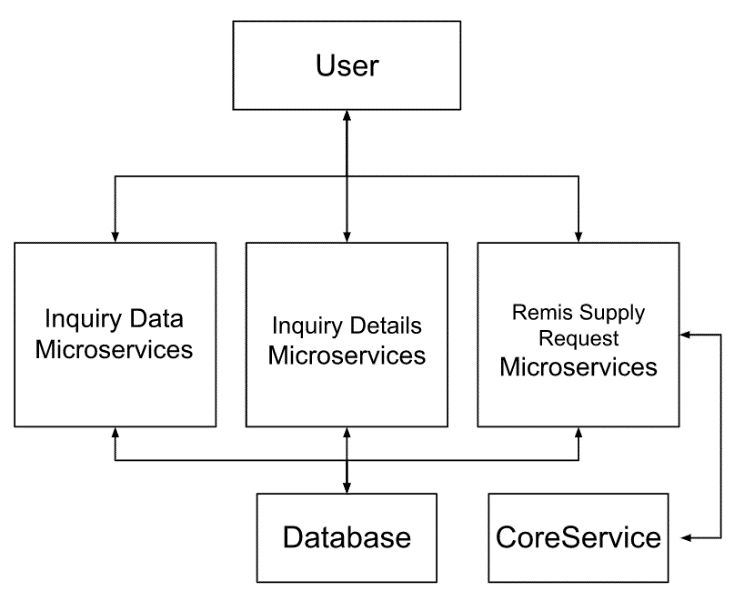
\includegraphics[width=0.5\linewidth]{imagens/maulana_scenario.jpg}    
    {\par \raggedright \footnotesize Fonte: \textcite{maulana_design_2022}.\par}
\end{figure}

Os testes de desempenho foram realizados para comparar as arquiteturas monolítica e de microsserviços sob diferentes condições de carga e estresse, incluindo variações no número de requisições simultâneas e cenários de alta (Ver \autoref{tab:3-maulana-testes-carga}) concorrência, utilizando o tempo de resposta, a latência e o \textit{throughput} como métricas principais. 

\begin{table}[H]
\centering
\caption{Condições de carga e estresse}
\label{tab:3-maulana-testes-carga}
\makebox[\textwidth][c]{%
\begin{tabularx}{\textwidth}{|l|X|}
\hline
\textbf{Condições de carga} & Throughput de 200 e 1.000 threads por minuto. \\
\hline
\textbf{Condições de estresse (microsserviços)} & \textit{Ramp-up} de 1 a 1.000 threads. \\
\hline
\end{tabularx}%
}
{\par \raggedright \footnotesize Fonte: \textcite{maulana_design_2022}.\par}
\end{table}

Na arquitetura monolítica, os resultados revelaram tempos distintos entre os subserviços: o serviço Remis Supply Request apresentou o maior tempo médio de resposta, de \textbf{1.616,06 ms}, devido à sua complexidade operacional, já mencionada no detalhamento dos serviços. Em seguida, o Inquiry Data registrou \textbf{389,65 ms} e o Inquiry Details, \textbf{241,175 ms}, como pode ser observado nas figuras \ref{fig:maulana_thp_mono} e \ref{fig:maulana_time_mono}. A latência e o \textit{throughput} variaram conforme a complexidade do fluxo de cada subserviço, impactando diretamente o desempenho do sistema monolítico.



\begin{figure}[htb]
  \centering
  \begin{minipage}[t]{0.48\linewidth}
    \caption{Throughput Cenário Monolítico}
    \label{fig:maulana_thp_mono}
    \centering
    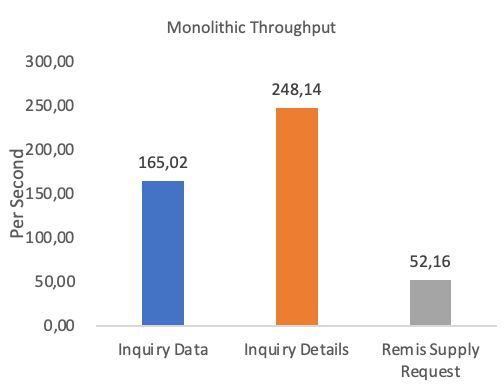
\includegraphics[width=\linewidth]{imagens/maulana_thp_mono.jpg}    
    {\par \raggedright \footnotesize Fonte: \textcite{maulana_design_2022}.\par}
  \end{minipage}%
  \hfill
  \begin{minipage}[t]{0.48\linewidth}
    \caption{Throughput Cenário Microsserviços}
    \label{fig:maulana_thp_ms}
    \centering
    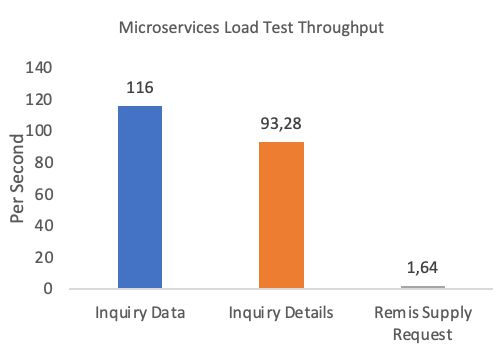
\includegraphics[width=\linewidth]{imagens/maulana_thp_ms.jpg}
    
    {\par \raggedright \footnotesize Fonte: \textcite{maulana_design_2022}.\par}
  \end{minipage}
\end{figure}

Em contraste, nos testes com a arquitetura de microsserviços, os tempos de resposta evidenciam diferenças significativas. O subserviço Remis Supply Request apresenta o maior tempo de resposta médio, de \textbf{4.240,4 ms}, superando consideravelmente o Inquiry Data, que registra \textbf{586 ms}, e o Inquiry Details, que alcança \textbf{552 ms} conforme ilustrado nas figuras \ref{fig:maulana_thp_ms} e \ref{fig:maulana_time_ms}. Os subserviços Inquiry Data e Inquiry Details demonstram resultados instáveis, com variações de desempenho e tendem a diminuir sob alta carga, sugerindo desafios na orquestração e na comunicação entre os novos serviços.

\begin{figure}[htb]
  \centering
  \begin{minipage}[t]{0.48\linewidth}
    \caption{Latência Cenário Monolítico}
    \label{fig:maulana_time_mono}
    \centering
    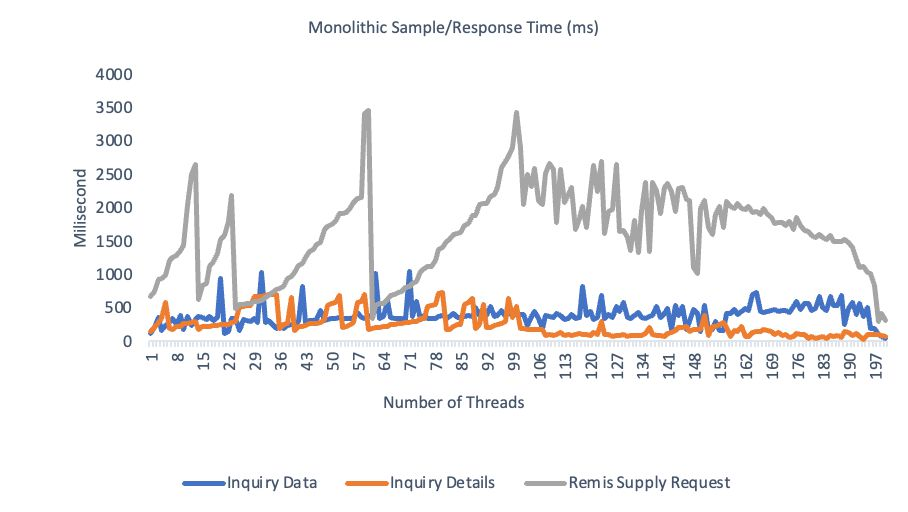
\includegraphics[width=\linewidth]{imagens/maulana_time_mono.jpg}    
    {\par \raggedright \footnotesize Fonte: \textcite{maulana_design_2022}.\par}
  \end{minipage}%
  \hfill
  \begin{minipage}[t]{0.48\linewidth}
    \caption{Latência Cenário Microsserviços}
    \label{fig:maulana_time_ms}
    \centering
    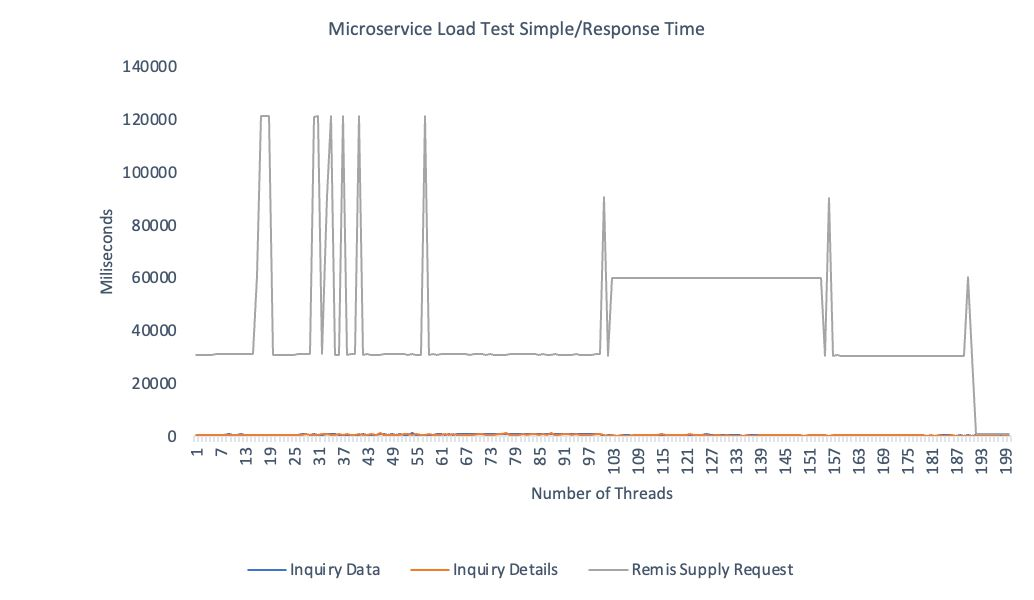
\includegraphics[width=\linewidth]{imagens/maulana_time_ms.jpg}    
    {\par \raggedright \footnotesize Fonte: \textcite{maulana_design_2022}.\par}
  \end{minipage}
\end{figure}

Além dos testes de carga, foram realizados cenários de stress testing para avaliar a capacidade da arquitetura de microsserviços em lidar com grandes volumes de requisições simultâneas. Os autores concluíram que, embora a arquitetura monolítica, executada em servidor on-premises (Intel® Xeon® CPU E5-2680 v3 @ 2.50GHz, 8GB \acrshort{ram} com Docker), tenha apresentado melhor desempenho em alguns testes específicos de tempo de resposta, a arquitetura de microsserviços, hospedada em máquina virtual no Google Compute Engine (n1-standard-2, Intel Haswell 1 vCPU, 7.5GB \acrshort{ram}) com Spring Boot, é preferível para desenvolvimento e manutenção. Isso decorre da simplicidade de gerenciamento, independência entre os subserviços e possibilidade de uso de diferentes tecnologias conforme a necessidade, aspectos inviáveis na arquitetura monolítica \cite{rademacher_modeling_2020}.

 \subsubsection{Resumo do Estudo}

Em síntese, o estudo de \textcite{maulana_design_2022} investigou a migração de um sistema bancário monolítico para microsserviços, com foco nos testes de desempenho em um contexto financeiro real. A pesquisa avaliou métricas como tempo de resposta, latência e \textit{throughput} em cenários de carga e estresse, destacando a capacidade dos microsserviços de atender às demandas de robustez e adaptabilidade do setor bancário. Os resultados indicaram que, embora o desempenho bruto em alguns testes específicos possa favorecer o sistema monolítico, em função das diferentes especificações de hardware utilizadas nos experimentos, a arquitetura de microsserviços é considerada superior para o desenvolvimento e a manutenção, devido à modularidade e à flexibilidade tecnológica. Essas características são cruciais para a agilidade e a inovação exigidas por bancos e outras instituições financeiras.

Contudo, uma limitação significativa do trabalho reside no fato de que os autores não investigaram diferentes formas de orquestração de microsserviços, focando exclusivamente na comparação entre arquiteturas monolítica e de microsserviços. Essa lacuna é particularmente relevante, pois a escolha do protocolo de comunicação entre microsserviços (\gls{rest}, \gls{grpc}, Apache Thrift, entre outros) pode impactar substancialmente o desempenho, a latência e a eficiência operacional do sistema, aspectos críticos para aplicações bancárias que demandam alta disponibilidade e tempos de resposta consistentes. A ausência de uma análise comparativa entre diferentes tecnologias de orquestração constitui uma oportunidade de pesquisa importante para aprofundar a compreensão sobre como otimizar a comunicação inter-serviços em ambientes financeiros distribuídos, reforçando a relevância da presente pesquisa no contexto da transformação digital do setor financeiro.

% -- Jhingran 2024
\subsection{Decentralized Generative AI Model Deployment Using Microservices \cite{jhingran_decentralized_2024}}
\label{subsec:jhingran_decentralized}

\textcite{jhingran_decentralized_2024} propõem uma solução para a implantação de modelos de \acrfull{ia} Generativa de forma descentralizada, utilizando uma arquitetura baseada em microsserviços. O estudo aborda os desafios inerentes à implantação de modelos complexos de \gls{ia} Generativa em sistemas centralizados, como gargalos de desempenho, falta de flexibilidade e dificuldades de escalabilidade. A motivação dos autores reside nas limitações dos sistemas centralizados, que frequentemente resultam em alta latência, comprometimento da integridade dos dados em situações de múltiplas requisições concorrentes \cite{lu_computing_2024}, além do considerável consumo de largura de banda e recursos computacionais. A pesquisa visa demonstrar como a abordagem descentralizada, habilitada por microsserviços, pode otimizar o uso de recursos, melhorar a tolerância a falhas e aumentar a escalabilidade, permitindo a distribuição da carga de trabalho entre múltiplos nós e reduzindo a latência ao processar dados mais próximos da "borda" da rede \cite{jhingran_performance_2021}.

A solução proposta consiste na divisão de modelos de \gls{ia} Generativa em componentes modulares, com cada módulo implementado como um microsserviço \cite{gustrowsky_using_2024}. Esses microsserviços comunicam-se por meio de \acrfull{api}s \gls{rest}, permitindo a execução em ambientes on-premise ou na nuvem. Essa distribuição da carga computacional tem como objetivo reduzir a latência e otimizar a largura de banda. O processo de implantação envolve etapas como o particionamento do modelo em submódulos, a conteinerização (com Docker), a implantação em nós distribuídos (com Kubernetes), o autoescalonamento, o balanceamento de carga, o monitoramento, a tolerância a falhas, a integração \acrfull{ci/cd} e considerações de segurança e privacidade dos dados.

A avaliação do desempenho da solução descentralizada foi realizada por meio de diversas métricas comparativas entre as abordagens centralizada e descentralizada. Os resultados, apresentados na  \autoref{tab:3-jhingran_performance_comparison}, destacam melhorias significativas em áreas como latência, utilização de largura de banda, tolerância a falhas, tempo de resposta, custo, consumo de energia e eficiência na utilização de computação.

\begin{table}[H]
\centering
\caption{Comparação entre Arquiteturas Centralizadas e Descentralizadas.}
\label{tab:3-jhingran_performance_comparison}
\begin{tabularx}{\textwidth}{| X | c | c | c | c |}
\hline
\textbf{Métrica} & \textbf{Monolítica} & \textbf{Microsserviços} & \textbf{Melhoria (\%)} & \textbf{Unidade} \\
\hline
Latência                  & 250ms   & 50ms    & 80 & ms \\
\hline
Uso de Banda              & 100GB   & 30GB    & 70 & GB \\
\hline
Tolerância a Falhas       & 60\%    & 95\%    & 35 & \% \\
\hline
Escalabilidade            & Média   & Alta    & N/A & Qualitativa \\
\hline
Tempo de Resposta         & 500ms   & 100ms   & 80 & ms \\
\hline
Consumo de Energia          & 3000W   & 1200W   & 60 & Watts \\
\hline
Acurácia do Modelo        & 90\%    & 92\%    & 2  & \% \\
\hline
\end{tabularx}
{\par \raggedright \footnotesize Fonte: \textcite{jhingran_decentralized_2024}\par}
\end{table}


A análise dos resultados demonstra claramente as vantagens da implantação dos modelos de \gls{ia} Generativa de forma descentralizada em microsserviços. Esses aspectos são especialmente relevantes para aplicações que exigem eficiência, custo-benefício e confiabilidade. Como pode ser observado na \autoref{tab:3-jhingran_performance_comparison}, a latência foi reduzida em\textbf{ 80\% (de 250 ms para 50ms)} e o tempo de resposta também diminuiu em \textbf{80\% (de 500 ms para 100 ms)}, o que melhora significativamente a experiência do usuário e possibilita processamento em tempo real. Além disso, a utilização da largura de banda apresentou uma melhoria de \textbf{70\%}, indicando menores custos de transferência de dados e maior velocidade no manuseio de informações.

Além disso, a tolerância a falhas aumentou em \textbf{35\%} e a escalabilidade foi classificada como alta, indicando que os sistemas descentralizados são mais resilientes a interrupções e falhas de modelo, o que eleva a confiabilidade e a disponibilidade do sistema. A eficiência de custos é notável, com uma redução de 70\% (de \$5000 para \$1500), o que torna a implantação descentralizada mais econômica para aplicações de \gls{ia} em larga escala. O \textbf{consumo de energia} foi reduzido em\textbf{ 60\%}, alinhando-se aos objetivos de sustentabilidade e diminuindo os custos operacionais. 

\subsubsection{Resumo do Estudo}

O estudo de \textcite{jhingran_decentralized_2024} demonstra experimentalmente as vantagens da implantação descentralizada de modelos de \gls{ia} Generativa em arquiteturas de microsserviços, apresentando melhorias substanciais em \textbf{latência (80\%)}, \textbf{custo (70\%)} e tolerância a \textbf{falhas (35\%)} em comparação com sistemas centralizados. A pesquisa apresenta uma abordagem prática para superar limitações de escalabilidade e recursos em sistemas de \gls{ia}, estabelecendo diretrizes para a implantação distribuída que otimiza o desempenho e a eficiência operacional.

Entretanto, o trabalho apresenta limitações metodológicas importantes que a pesquisa busca endereçar. Enquanto \textcite{jhingran_decentralized_2024} focam em comparações teóricas entre arquiteturas centralizadas e descentralizadas sem especificar protocolos de comunicação ou validação experimental controlada, a investigação preenche essa lacuna ao comparar empiricamente protocolos específicos (\gls{rest}, \gls{grpc}, Apache Thrift) em cenários reais de assistentes virtuais multimodais no setor financeiro. Adicionalmente, a abordagem considera não apenas métricas de desempenho geral, mas também aspectos críticos como latência de cauda (p95, p99) e eficiência de recursos sob diferentes complexidades de processamento de \gls{ia}, oferecendo diretrizes práticas para decisões arquiteturais em domínios de alta criticidade.


\section{Síntese do Capítulo}
\label{sec:sintese_capitulo}

Neste capítulo, foi apresentada uma \acrfull{rsl}, conduzida segundo as diretrizes de \cite{scannavino_revisao_2017}, detalhando bases de dados, estratégias de busca e critérios de seleção para assegurar a qualidade científica dos estudos relacionados à orquestração de microsserviços e \gls{ia} Generativa no setor financeiro.

A análise dos trabalhos revelou três vertentes principais de pesquisa: \textcite{niswar_performance_2024} estabeleceram a superioridade do \gls{grpc} sobre \gls{rest} e \acrshort{graphql} em cenários genéricos, mas sem considerar cargas de \gls{ia} generativa; \textcite{maulana_design_2022} demonstraram a viabilidade da migração para microsserviços no setor bancário, porém sem especificar protocolos de comunicação ou métricas de latência de cauda; e \textcite{jhingran_decentralized_2024} propuseram vantagens teóricas da descentralização em \gls{ia} generativa, mas sem validação experimental controlada.

Esta pesquisa preenche lacunas identificadas ao combinar aspectos dos três trabalhos: a comparação rigorosa de protocolos de comunicação (expandindo para incluir Apache Thrift), o foco específico no setor financeiro (com requisitos de latência críticos), e a aplicação prática em sistemas de \gls{ia} generativa multimodal (validada experimentalmente). A contribuição, conforme comparada na \autoref{tab:posicionamento_estado_arte}, se posiciona como a primeira investigação experimental abrangente sobre orquestração de microsserviços para assistentes virtuais multimodais no contexto financeiro, oferecendo diretrizes práticas baseadas em evidências empíricas para decisões arquiteturais em um domínio de alta criticidade.

\begin{table}[htbp]
\centering
\caption{Posicionamento deste trabalho no Estado da Arte}
\label{tab:posicionamento_estado_arte}
\makebox[\textwidth]{%
\begin{tabularx}{1.2\textwidth}{|l|X|X|X|X|}
\hline
\textbf{Aspecto} & \textbf{\textcite{niswar_performance_2024}} & \textbf{\textcite{maulana_design_2022}} & \textbf{\textcite{jhingran_decentralized_2024}} & \textbf{Esta Dissertação} \\
\hline
Domínio de Aplicação & Sistema Educacional & Sistema Bancário Genérico & \gls{ia} Generativa Genérica & \textbf{Assistentes Virtuais Financeiros Multimodais} \\
\hline
Protocolos Comparados & \gls{rest}, \acrshort{graphql}, \gls{grpc} & Monolítico vs Microsserviços & Centralizado vs Descentralizado & \textbf{\gls{rest}, \gls{grpc}, Apache Thrift} \\
\hline
Ambiente de Teste & Dados estáticos & Migração real limitada & Teórico/simulado & \textbf{Ambiente controlado com \gls{ia} real} \\
\hline
Métricas de Latência & Tempo médio de resposta & Tempo de resposta básico & Comparação teórica & \textbf{p50, p95, p99 + máximos} \\
\hline
Complexidade dos Cenários & Dados planos vs aninhados & Carga única & Não especificado & \textbf{Simples, Tradicional, Complexo} \\
\hline
Foco em \gls{ia} Generativa & Não & Não & Sim (Teórico) & \textbf{Sim (Experimental)} \\
\hline
Setor Financeiro & Não & Sim (Genérico) & Não & \textbf{Sim (Específico)} \\
\hline
Tamanho Amostral & Limitado & Caso único & N/A & \textbf{15 replicações × 3 cenários × 3 protocolos} \\
\hline
Multimodalidade & Não & Não & Sim (\gls{llm}) & \textbf{Sim (\gls{stt}, \gls{llm} e \gls{tts})} \\
\hline
\end{tabularx}%
}
{\par \raggedright \footnotesize Fonte: Elaborado pelo autor.\par}
\end{table}

